\addtotoc{English Summary}
\thispagestyle{plain}

% Tovchlol figures/tables are excluded from the global lists
\captionsetup{list=no}

% English caption labels for this section
\renewcommand{\figurename}{Figure}
\renewcommand{\tablename}{Table}

\vspace*{-6mm}
\begin{center}
\textbf{\large FOREIGN EXCHANGE TRADING SIGNAL GENERATION SYSTEM}\\[1mm]
\end{center}

\begin{flushright}
Department of Computer Science\\
Student: \studentID, M.~Munkhdorj\\
Supervisor: N.~Soronzonbold
\end{flushright}

\vspace{1mm}
\setcounter{table}{0}
\setcounter{figure}{0}
\renewcommand{\thetable}{\arabic{table}}
\renewcommand{\thefigure}{\arabic{figure}}
\setlength{\columnsep}{7mm}
\begin{multicols*}{2}
\setlength{\parskip}{4pt}
\setlength{\intextsep}{4pt}
\setlength{\textfloatsep}{4pt}
\setlength{\abovecaptionskip}{2pt}
\setlength{\belowcaptionskip}{2pt}
\sloppy

%%─────────────────────────────────────────────
\noindent\textbf{1. Introduction}

The foreign exchange (Forex) market produces highly volatile, noisy time series, so forecasting based on traditional statistical methods remains limited. Although GBDT and neural-network models have been shown capable of detecting patterns, single-model architectures are still hindered in practice by the risk of overfitting. This study builds a GBDT-ensemble ML system that generates BUY/HOLD/SELL classification signals for the EUR/USD pair and delivers them to users through a mobile application. Three research questions were posed:
\begin{itemize}\setlength\itemsep{0pt}\small
    \item \textbf{RQ1:} Does the model perform reliably on a chronologically ordered hold-out test?
    \item \textbf{RQ2:} Do the filtered signals actually execute as real trades?
    \item \textbf{RQ3:} Under a fixed-risk rule, does the system yield a positive return over one year?
\end{itemize}

%%─────────────────────────────────────────────
\noindent\textbf{2. Background and Related Work}

Research on financial time-series forecasting developed amid the theoretical skepticism of the Efficient Market Hypothesis (EMH), yet recent years have reinforced that machine learning can detect patterns to a meaningful degree. Krauss et al.\ (2017) concluded that GBDT yields more reliable results than deep learning, while Ballings et al.\ (2015) found that ensembles gain 3--7\% over single models. Although Fischer \& Krauss (2018) tested LSTM on the S\&P~500 and Yildirim et al.\ (2021) on EUR/USD, empirical work combining multi-timeframe feature engineering with a GBDT ensemble remains scarce.

\emph{Contribution.} This study empirically tests, within a single unified system, a GBDT ensemble, multi-timeframe features, confidence-threshold signal filtering, and a mobile interface for the Forex market.

%%─────────────────────────────────────────────
\noindent\textbf{3. Methodology}

An ML serving system spanning from model training to the mobile app was built (Figure~\ref{fig:toven_system_architecture}). It has three core layers: (i)~offline training (GBDT pkl); (ii)~Server (Flask + MongoDB + Redis + Expo Push) + 4 external APIs; (iii)~Mobile app (React Native, 4 screens).

\begin{figure}[H]
\centering
\adjustbox{max width=\columnwidth}{%
\begin{tikzpicture}[
    vm/.style={rectangle, rounded corners=5pt, draw=orange!85!black, fill=orange!22,
               line width=1.1pt, minimum width=4.8cm, minimum height=1.4cm,
               align=center, font=\normalsize\bfseries, inner sep=5pt},
    plainbox/.style={rectangle, rounded corners=4pt, draw=black!75, fill=white,
                     line width=1.0pt, minimum width=2.8cm, minimum height=1.0cm,
                     align=center, font=\normalsize, inner sep=4pt},
    websvc/.style={rectangle, rounded corners=5pt, draw=red!70!black, fill=red!25,
                   line width=1.0pt, minimum width=2.9cm, minimum height=1.0cm,
                   align=center, font=\normalsize\bfseries, text=black!85, inner sep=4pt},
    db/.style={cylinder, shape border rotate=90, aspect=0.30,
               draw=blue!65, fill=blue!18, line width=1.0pt,
               minimum width=2.4cm, minimum height=1.2cm,
               align=center, font=\normalsize\bfseries, text=blue!25!black},
    extapi/.style={rectangle, rounded corners=5pt, draw=green!55!black, fill=green!15,
                   line width=1.0pt, minimum width=3.0cm, minimum height=1.0cm,
                   align=center, font=\normalsize\bfseries, inner sep=4pt},
    pushsvc/.style={rectangle, rounded corners=5pt, draw=violet!70!black, fill=violet!18,
                    line width=1.0pt, minimum width=2.8cm, minimum height=1.1cm,
                    align=center, font=\normalsize\bfseries, inner sep=4pt},
    userbox/.style={rectangle, minimum width=0.9cm, minimum height=1.5cm,
                    draw=none, fill=none, inner sep=0pt},
    stickline/.style={line width=1.1pt, color=black!75, line cap=round},
    pipebox/.style={rectangle, rounded corners=4pt, draw=teal!60!black, fill=teal!14,
                    line width=1.0pt, minimum width=2.9cm, minimum height=1.0cm,
                    align=center, font=\normalsize, inner sep=4pt},
    flowarr/.style={-{Stealth[length=5pt 1.5, width'=0pt 0.6, sep=0pt 0.5]},
                    line width=1.0pt, color=black!72,
                    rounded corners=4pt, shorten >=2pt},
    thinarr/.style={-{Stealth[length=4pt 1.5, width'=0pt 0.6, sep=0pt 0.5]},
                    line width=0.7pt, color=black!60,
                    rounded corners=4pt, shorten >=2pt},
    busline/.style={line width=1.0pt, color=black!72},
    pusharr/.style={-{Stealth[length=5pt 1.5, width'=0pt 0.6, sep=0pt 0.5]},
                    line width=1.0pt, densely dashed, color=violet!65!black,
                    rounded corners=4pt, shorten >=2pt},
    deparr/.style={-{Triangle[open, length=4mm, width=3mm]},
                   line width=1.0pt, dashed, color=teal!55!black,
                   rounded corners=4pt, shorten >=2pt},
    elabel/.style={font=\small, text=black!65, fill=white, inner sep=1.5pt},
]
\node[userbox] (users) at (-9, 5.5) {};
\draw[stickline] ($(users.center)+(0, 0.46)$) circle (0.17);
\draw[stickline] ($(users.center)+(0, 0.29)$) -- ($(users.center)+(0, -0.25)$);
\draw[stickline] ($(users.center)+(-0.30, 0.08)$) -- ($(users.center)+(0.30, 0.08)$);
\draw[stickline] ($(users.center)+(0, -0.25)$) -- ($(users.center)+(-0.22, -0.65)$);
\draw[stickline] ($(users.center)+(0, -0.25)$) -- ($(users.center)+(0.22, -0.65)$);
\node[font=\small\bfseries, anchor=north] at ($(users.south)+(0, 0.05)$) {Users};
\node[plainbox] (mob)  at (-4, 5.5) {Mobile app\\[1pt]{\small (React Native)}};
\node[pushsvc]  (expo) at ( 0, 5.5) {Expo Push};
\draw[flowarr] (users.east) -- (mob.west);
\node[plainbox] (dns) at (-4, 3.5) {DNS};
\draw[flowarr] (mob.south) -- (dns.north);
\draw[black!55, line width=1.2pt, rounded corners=10pt]
    (-7, -5.6) rectangle (1, 2.4);
\node[font=\large\bfseries, anchor=north west, text=black!72]
    at (-6.85, 2.32) {Server};
\node[vm] (api)    at (-4,  0.9) {API server\\[1pt]{\small Flask + Gunicorn}};
\node[vm] (worker) at (-4, -1.6) {Worker\\[1pt]{\small Inference $\cdot$ Processing}};
\draw[flowarr] (dns.south)  -- (api.north);
\draw[flowarr] (api.south)  -- (worker.north);
\node[plainbox] (cache) at (-5.3, -4.2) {Cache\\[1pt]{\small (Redis)}};
\node[db]       (mongo) at (-1.7, -4.4) {MongoDB};
\coordinate (db_trunk) at (-4, -2.7);
\draw[busline]  (worker.south) -- (db_trunk);
\draw[flowarr] (db_trunk) -| (cache.north);
\draw[flowarr] (db_trunk) -| (mongo.north);
\draw[thinarr] (cache.east) -- (-2.9, -4.2);
\fill[red!4, rounded corners=8pt]   (-12, -3.1) rectangle (-8, 1.95);
\draw[red!50, line width=0.8pt, rounded corners=8pt]
    (-12, -3.1) rectangle (-8, 1.95);
\node[font=\small\bfseries, anchor=north, text=red!55!black]
    at (-10, 1.85) {Internal services};
\node[websvc] (mail)  at (-10,  0.9) {Email};
\node[websvc] (queue) at (-10, -1.1) {Job\\queue};
\node[websvc] (mon)   at (-10, -2.1) {Monitoring};
\draw[thinarr] (mail.east) -- (api.west);
\draw[thinarr] (queue.east) -- ([yshift= 0.5cm]worker.west);
\draw[thinarr] (mon.east) -- ([yshift=-0.5cm]worker.west);
\fill[green!4, rounded corners=8pt]   (2.5, -2.9) rectangle (7.6, 3.2);
\draw[green!45!black, line width=0.8pt, rounded corners=8pt]
    (2.5, -2.9) rectangle (7.6, 3.2);
\node[font=\small\bfseries, anchor=north, text=green!40!black]
    at (5.05, 3.1) {Third-party APIs};
\node[extapi] (yf)  at (5.05,  1.9) {Yahoo Finance};
\node[extapi] (av)  at (5.05,  0.7) {AlphaVantage};
\node[extapi] (tv)  at (5.05, -0.5) {TradingView};
\node[extapi] (gem) at (5.05, -1.6) {Gemini API};
\draw[busline] (3.2, 1.9) -- (3.2, -1.6);
\draw[busline] (yf.west)  -- (3.2,  1.9);
\draw[busline] (av.west)  -- (3.2,  0.7);
\draw[busline] (tv.west)  -- (3.2, -0.5);
\draw[busline] (gem.west) -- (3.2, -1.6);
\node[circle, fill=black!72, minimum size=4pt, inner sep=0pt] at (3.2, -1.6) {};
\draw[flowarr] (3.2, -1.6) -- (worker.east);
\draw[pusharr] ([yshift=0.5cm]worker.east) -- ++(0.5, 0) -| (expo.south);
\draw[pusharr] (expo.west) -- (mob.east);
\fill[teal!4, rounded corners=8pt]   (-7, -8.7) rectangle (5, -6.5);
\draw[teal!50!black, line width=0.8pt, rounded corners=8pt]
    (-7, -8.7) rectangle (5, -6.5);
\node[font=\small\bfseries, anchor=north, text=teal!40!black]
    at (-1, -6.6) {Offline training};
\node[pipebox] (csv)   at (-5, -7.7) {Historical data};
\node[pipebox] (train) at (-1, -7.7) {GBDT training};
\node[pipebox] (pkl)   at ( 3, -7.7) {model.pkl};
\draw[flowarr] (csv.east)   -- (train.west);
\draw[flowarr] (train.east) -- (pkl.west);
\node[elabel] at ([yshift=32pt, xshift=-20pt]pkl.north) {deploy};
\draw[deparr] (pkl.north) |- (1.5, -6.3) |- ([yshift=-0.5cm]worker.east);
\end{tikzpicture}%
}
\caption{System architecture}
\label{fig:toven_system_architecture}
\end{figure}

\emph{Data.} A 48-feature matrix was built from EUR/USD 2015--2024 historical data over 6 timeframes (M1--H4) $\times$ 8 technical indicators. Labels were assigned to BUY/SELL/HOLD by a 30-pip threshold on the future 240-minute move.

\emph{Model.} LightGBM, XGBoost, and CatBoost were combined by equal-weight soft voting (Figure~\ref{fig:toven_ensemble_arch}). The three models complement one another through different growth strategies (leaf-wise, level-wise, symmetric), reducing the risk of overfitting. Training used the fifth WFV fold (train 2015--2022, val 2023, test 2024). Six anti-overfitting measures were combined: limited tree depth, low learning rate, early stopping, L1/L2 regularization, WFV, and feature selection.

\begin{figure}[H]
\centering
\adjustbox{max width=\columnwidth}{%
\begin{tikzpicture}[
    inp/.style ={rectangle, rounded corners=4pt, draw=blue!65, fill=blue!18,
                 line width=1.0pt, minimum width=6.0cm, minimum height=1.0cm,
                 align=center, font=\small\bfseries, text=blue!25!black},
    lgbm/.style={rectangle, rounded corners=4pt, draw=orange!85!black, fill=orange!22,
                 line width=1.0pt, minimum width=3.4cm, minimum height=1.25cm,
                 align=center, font=\small\bfseries, text=black!82},
    xgb/.style ={rectangle, rounded corners=4pt, draw=green!55!black, fill=green!15,
                 line width=1.0pt, minimum width=3.4cm, minimum height=1.25cm,
                 align=center, font=\small\bfseries, text=black!82},
    cat/.style ={rectangle, rounded corners=4pt, draw=teal!60!black, fill=teal!14,
                 line width=1.0pt, minimum width=3.4cm, minimum height=1.25cm,
                 align=center, font=\small\bfseries, text=black!82},
    vote/.style={rectangle, rounded corners=4pt, draw=violet!70!black, fill=violet!18,
                 line width=1.1pt, minimum width=6.0cm, minimum height=1.2cm,
                 align=center, font=\small\bfseries, text=black!82},
    outp/.style={rectangle, rounded corners=4pt, draw=red!70!black, fill=red!25,
                 line width=1.1pt, minimum width=3.4cm, minimum height=1.0cm,
                 align=center, font=\small\bfseries, text=black!85},
    sigb/.style={rectangle, rounded corners=4pt, draw=red!70!black, fill=red!25,
                 line width=1.1pt, minimum width=7.2cm, minimum height=1.0cm,
                 align=center, font=\small\bfseries, text=black!85},
    arr/.style ={-{Stealth[length=5pt 1.5, width'=0pt 0.6, sep=0pt 0.5]},
                 line width=1.0pt, color=black!72},
    lin/.style ={line width=1.0pt, color=black!72},
    lbl/.style ={font=\scriptsize\bfseries, fill=white, inner sep=1pt, text=black!65},
]
\node[inp]  (X)   at (0,  0)    {48 features};
\node[lgbm] (lgb) at (-4, -2.4) {LightGBM};
\node[xgb]  (xgb) at ( 0, -2.4) {XGBoost};
\node[cat]  (cat) at ( 4, -2.4) {CatBoost};
\node[vote] (avg) at (0, -5.2)  {Soft voting\\$\bar{p}_c = \tfrac{1}{3}\sum_i p_i^{(c)},\ c\in\{$BUY,HOLD,SELL$\}$};
\node[sigb] (sig)    at (0, -7.4)    {Trading signal (BUY / HOLD / SELL, confidence $\in [0,1]$)};

\draw[arr] (X.south) -- (lgb.north);
\draw[arr] (X.south) -- (xgb.north);
\draw[arr] (X.south) -- (cat.north);

\coordinate (bus) at (0, -4.3);
\draw[lin] (lgb.south) -- ++(0, -0.4) -| (bus);
\draw[lin] (xgb.south) -- (bus);
\draw[lin] (cat.south) -- ++(0, -0.4) -| (bus);
\node[lbl, text=orange!85!black] at ($(lgb.south) + (0.35,-0.2)$) {$p_1$};
\node[lbl, text=green!55!black]  at ($(xgb.south) + (0.35,-0.2)$) {$p_2$};
\node[lbl, text=teal!60!black]   at ($(cat.south) + (0.35,-0.2)$) {$p_3$};
\draw[arr] (bus) -- (avg.north);

\draw[arr] (avg.south) -- (sig.north);
\end{tikzpicture}%
}
\caption{GBDT ensemble model architecture}
\label{fig:toven_ensemble_arch}
\end{figure}

\emph{Signal filter.} Signals are filtered by confidence (conf~$\geq 0.90$) and ATR (~$\geq 4$ pips); of 359{,}639 predictions in 2025, 3{,}567 (1.0\%) remained, and MT5's \texttt{MaxPositions=1} rule executed 230 trades (Figure~\ref{fig:toven_signal_funnel}). SL/TP are computed dynamically from ATR with a 3:1 TP/SL ratio.

\begin{figure}[H]
\centering
\adjustbox{max width=\columnwidth}{%
\begin{tikzpicture}[
    cnt/.style={font=\small\bfseries, text=black!82},
    pct/.style={font=\scriptsize, text=black!65},
    arr/.style={-{Stealth[length=5pt 1.5, width'=0pt 0.6, sep=0pt 0.5]},
                line width=1.0pt, color=black!72},
]
\node[trapezium, trapezium angle=78, trapezium stretches body,
      shape border rotate=180,
      draw=blue!65, fill=blue!18, line width=1.0pt,
      minimum height=1.0cm, minimum width=12cm,
      align=center, font=\small\bfseries, text=blue!25!black] (s1) at (0, 0)
    {1. Total predictions (GBDT ensemble, 2025)};
\node[cnt, right=0.5cm of s1] {359{,}639};
\node[pct, right=2.4cm of s1] {(100\%)};
\node[trapezium, trapezium angle=78, trapezium stretches body,
      shape border rotate=180,
      draw=orange!85!black, fill=orange!22, line width=1.0pt,
      minimum height=1.0cm, minimum width=8cm,
      align=center, font=\small\bfseries, text=black!82,
      below=0.5cm of s1] (s2)
    {2. Confidence $\geq 0.90$ filter};
\node[cnt, right=0.5cm of s2] {$\sim$3{,}600};
\node[pct, right=2.2cm of s2] {($\approx$1.00\%)};
\node[trapezium, trapezium angle=78, trapezium stretches body,
      shape border rotate=180,
      draw=orange!85!black, fill=orange!22, line width=1.0pt,
      minimum height=1.0cm, minimum width=5.5cm,
      align=center, font=\small\bfseries, text=black!82,
      below=0.5cm of s2] (s3)
    {3. ATR $\geq 4.0$ pips filter};
\node[cnt, right=0.5cm of s3] {3{,}567};
\node[pct, right=2.0cm of s3] {(0.99\%)};
\node[trapezium, trapezium angle=78, trapezium stretches body,
      shape border rotate=180,
      draw=teal!60!black, fill=teal!14, line width=1.0pt,
      minimum height=1.0cm, minimum width=3.6cm,
      align=center, font=\small\bfseries, text=black!82,
      below=0.5cm of s3] (s4)
    {4. MaxPositions=1\\\scriptsize\itshape(MT5 EA execution rule)};
\node[cnt, right=0.5cm of s4] {230};
\node[pct, right=1.6cm of s4] {(0.064\%)};
\node[rectangle, draw=red!70!black, fill=red!25, rounded corners=5pt,
      line width=1.1pt, minimum width=2.6cm, minimum height=0.9cm,
      align=center, font=\small\bfseries, text=black!85,
      below=0.5cm of s4] (s5)
    {5. Closed trades};
\node[cnt, right=0.5cm of s5] {230};
\node[pct, right=1.6cm of s5] {(TP: 103 / SL: 127)};
\draw[arr] (s1.south) -- (s2.north);
\draw[arr] (s2.south) -- (s3.north);
\draw[arr] (s3.south) -- (s4.north);
\draw[arr] (s4.south) -- (s5.north);
\node[pct, left=0.3cm of s2] {$-99.00\%$};
\node[pct, left=0.3cm of s3] {$-0.92\%$};
\node[pct, left=0.3cm of s4] {$-93.55\%$ (overlap)};
\end{tikzpicture}%
}
\caption{Signal filtering funnel (0.90 threshold)}
\label{fig:toven_signal_funnel}
\end{figure}

\emph{Experiment.} MT5 Strategy Tester, 2025.01--2026.01, \$10{,}000 initial capital, one position at a time, real spread + 10~point slippage, 10 confidence thresholds (0.90--0.99).

%%─────────────────────────────────────────────
\noindent\textbf{4. Results}

\emph{Classification quality.} On the unseen 2024 test set, overall accuracy reached \textbf{89.25\%} (all classes), while on the validation (2023) sample after conf~$\geq 0.90$ filtering accuracy rose to \textbf{96.96\%}. The validation--training gap of +1.77\% indicates no overfitting (Table~\ref{tab:toven_model_accuracy}).

\begin{table}[H]
\centering
\caption{GBDT ensemble accuracy and F1 scores}
\label{tab:toven_model_accuracy}
\scriptsize
\renewcommand{\arraystretch}{1.15}
\setlength{\tabcolsep}{3pt}
\begin{tabular}{|l|c|r|r|r|}
\hline
Split & Window & Acc (\%) & F1-mac & F1-wgt \\ \hline
Train               & 2015--2022 & 82.71 & 67.74 & 80.94 \\ \hline
Validation          & 2023       & 84.48 & 62.67 & 82.29 \\ \hline
Test (out-of-sample) & 2024      & \textbf{89.25} & \textbf{59.45} & \textbf{87.23} \\ \hline
\end{tabular}
\end{table}

\emph{Strategy return.} All 10 confidence thresholds (0.90--0.99) produced positive returns, beating the Buy~\&~Hold (+13.47\%) benchmark by 5.5--38$\times$. The 0.91 threshold reached the highest \textbf{+517.70\% (\$61{,}770)}, and the 0.90--0.92 band combined high return with low drawdown (MaxDD $<$~3\%), forming a balanced operating point (Figure~\ref{fig:toven_threshold_final_balance}).

\begin{figure}[H]
\centering
\adjustbox{max width=\columnwidth}{%
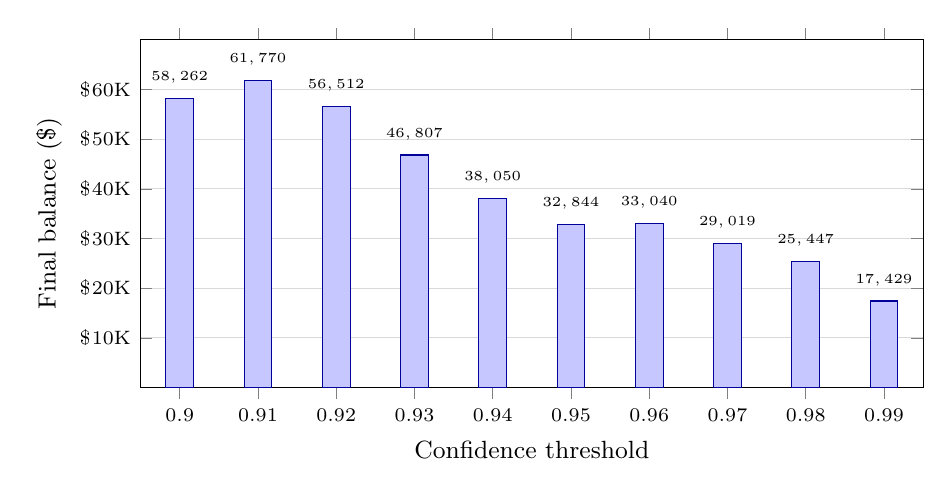
\begin{tikzpicture}
\begin{axis}[
    width=0.95\textwidth,
    height=6.0cm,
    ybar,
    bar width=10pt,
    xlabel={Confidence threshold},
    ylabel={Final balance (\$)},
    xmin=0.895, xmax=0.995,
    ymin=0, ymax=70000,
    xtick={0.90,0.91,0.92,0.93,0.94,0.95,0.96,0.97,0.98,0.99},
    ytick={10000,20000,30000,40000,50000,60000},
    yticklabels={\$10K, \$20K, \$30K, \$40K, \$50K, \$60K},
    scaled y ticks=false,
    ymajorgrids=true,
    grid style={gray!30},
    tick label style={font=\scriptsize},
    label style={font=\small},
    legend style={at={(0.98,0.97)},anchor=north east,font=\scriptsize,draw=gray!40,fill=white},
    area legend,
    nodes near coords,
    nodes near coords style={font=\tiny,yshift=2pt,/pgf/number format/.cd,fixed,precision=0,1000 sep={,}}
]
\addplot[fill=blue!22, draw=blue!60!black] coordinates {
    (0.90,58262) (0.91,61770) (0.92,56512) (0.93,46807) (0.94,38050)
    (0.95,32844) (0.96,33040) (0.97,29019) (0.98,25447) (0.99,17429)
};
\end{axis}
\end{tikzpicture}%
}
\caption{Final balance by threshold}
\label{fig:toven_threshold_final_balance}
\end{figure}

\emph{Risk and statistics.} Win rate 44.78--65.71\% (Wilson 95\% CI); binomial test $z>5$, $p<0.0001$; $E[R]$=0.79--1.63R, all positive; MaxDD 1.98--9.53\% (Figure~\ref{fig:toven_risk_smallmult}). The Sharpe values of 8.6--12.8 are \emph{inflated} by the small sample size, the short window, and the incomplete cost modeling, so they are valid only for relative comparison across thresholds.

\begin{figure}[H]
\centering
\adjustbox{max width=\columnwidth}{%
\pgfplotsset{
    smallpanel/.style={
        width=7.2cm, height=4.4cm,
        xmin=0.895, xmax=0.995,
        xtick={0.90,0.92,0.94,0.96,0.98},
        tick label style={font=\tiny},
        label style={font=\scriptsize},
        title style={font=\scriptsize,yshift=-2pt},
        ymajorgrids=true, grid style={gray!30},
        ybar, bar width=4.5pt,
    }
}
\begin{tabular}{@{}cc@{}}
\begin{tikzpicture}
\begin{axis}[smallpanel, title={(A) MaxDD (\%)}, ylabel={MaxDD (\%)}, ymin=0, ymax=10.5]
\addplot[fill=red!28, draw=red!60!black] coordinates {
    (0.90,3.93) (0.91,2.97) (0.92,2.99) (0.93,9.53) (0.94,6.80)
    (0.95,3.94) (0.96,4.88) (0.97,2.96) (0.98,7.66) (0.99,1.98)};
\end{axis}
\end{tikzpicture} &
\begin{tikzpicture}
\begin{axis}[smallpanel, title={(B) Sharpe}, ylabel={Sharpe}, ymin=0, ymax=14]
\addplot[fill=blue!28, draw=blue!60!black] coordinates {
    (0.90,9.11) (0.91,9.75) (0.92,9.90) (0.93,9.21) (0.94,8.87)
    (0.95,8.57) (0.96,9.84) (0.97,9.02) (0.98,10.63) (0.99,12.83)};
\end{axis}
\end{tikzpicture} \\[4pt]
\begin{tikzpicture}
\begin{axis}[smallpanel, title={(C) Sortino}, ylabel={Sortino}, ymin=0, ymax=48]
\addplot[fill=teal!28, draw=teal!60!black] coordinates {
    (0.90,24.82) (0.91,25.99) (0.92,29.78) (0.93,25.92) (0.94,24.66)
    (0.95,23.97) (0.96,30.15) (0.97,24.90) (0.98,28.84) (0.99,44.76)};
\end{axis}
\end{tikzpicture} &
\begin{tikzpicture}
\begin{axis}[smallpanel, title={(D) Calmar = Return / MaxDD}, ylabel={Calmar}, ymin=0, ymax=190]
\addplot[fill=orange!30, draw=orange!72!black] coordinates {
    (0.90,122.96) (0.91,174.20) (0.92,155.79) (0.93,38.63) (0.94,41.23)
    (0.95,57.97) (0.96,47.18) (0.97,64.19) (0.98,20.16) (0.99,37.53)};
\end{axis}
\end{tikzpicture}
\end{tabular}%
}
\caption{Risk metrics by threshold}
\label{fig:toven_risk_smallmult}
\end{figure}

%%─────────────────────────────────────────────
\noindent\textbf{5. Conclusion}

This study integrated a GBDT ensemble, confidence-threshold filtering, and a mobile interface for the EUR/USD market within an end-to-end pipeline from training to user, and tested it empirically. The three research questions were answered as follows:

\begin{itemize}\setlength\itemsep{0pt}\small
    \item \textbf{RQ1}: 89.25\% (test 2024, all classes) / 96.96\% (val 2023, conf~$\geq 0.90$)
    \item \textbf{RQ2}: 3{,}567 signals $\to$ 230 trades (6.45--23.81\%)
    \item \textbf{RQ3}: +74--518\% return, $E[R]$=0.79--1.63R
\end{itemize}

The top 3 thresholds by composite score (Table~\ref{tab:toven_rq3_summary}):

\begin{table}[H]
\centering
\caption{Top 3 thresholds by composite score}
\label{tab:toven_rq3_summary}
\scriptsize
\renewcommand{\arraystretch}{1.12}
\setlength{\tabcolsep}{2.5pt}
\begin{tabular}{|c|r|r|r|l|}
\hline
Threshold & Return & MaxDD & Win & Profile \\ \hline
0.91 & +517.70\% & 2.97\% & 47.17\% & \#1 Balanced \\ \hline
0.92 & +465.12\% & 2.99\% & 47.26\% & \#2 Balanced \\ \hline
0.99 & +74.29\%  & 1.98\% & 65.71\% & \#3 Risk-averse \\ \hline
\end{tabular}
\end{table}

Beyond statistical accuracy, the results validate the quality of an integrated pipeline: data collection~$\to$~feature engineering~$\to$~ensemble training~$\to$~signal filtering~$\to$~automated trade~$\to$~mobile notification. Scientifically, it presents empirical evidence combining a GBDT ensemble, multi-timeframe features, and confidence-threshold filtering; practically, it delivers a complete reference system from training to mobile distribution and demonstrates its ability to operate under real-time conditions.

\emph{Limitations.} The results are validated only for EUR/USD and the 2025 window, so they cannot be directly generalized to other pairs; commission and swap are not fully modeled; the signal-to-execution conversion is below 100\%.

\emph{Future work.} Extend to GBP/USD and USD/JPY; compare with LSTM/Transformer; manage position sizing via reinforcement learning (RL); implement a Model Registry and Google Play distribution.

%%─────────────────────────────────────────────
\noindent\textbf{References}

\begingroup
\scriptsize
\setlength{\parskip}{2pt}
\begin{enumerate}\setlength\itemsep{1pt}\setlength\parsep{0pt}\setlength\topsep{0pt}
    \item Krauss, C., Do, X.A., Huck, N. (2017). Deep Neural Networks, Gradient-Boosted Trees, Random Forests: Statistical Arbitrage on the S\&P~500. \emph{European Journal of Operational Research}, 259(2): 689--702.
    \item Ballings, M., Van den Poel, D., Hespeels, N., Gryp, R. (2015). Evaluating Multiple Classifiers for Stock Price Direction Prediction. \emph{Expert Systems with Applications}, 42(20): 7046--7056.
    \item Fischer, T., Krauss, C. (2018). Deep Learning with Long Short-Term Memory Networks for Financial Market Predictions. \emph{European Journal of Operational Research}, 270(2): 654--669.
    \item Ke, G., Meng, Q., Finley, T., Wang, T., Chen, W., Ma, W., Ye, Q., Liu, T.-Y. (2017). LightGBM: A Highly Efficient Gradient Boosting Decision Tree. \emph{Advances in Neural Information Processing Systems (NeurIPS)}, 30: 3146--3154.
    \item Yildirim, D.C., Toroslu, I.H., Fiore, U. (2021). Forecasting Directional Movement of Forex Data Using LSTM with Technical and Macroeconomic Indicators. \emph{Financial Innovation}, 7(1).
\end{enumerate}
\endgroup

\end{multicols*}
